
\chapter{Physics performance studies}
\label{cha:performance}

Below we describe the simulation studies performed to evaluate the impact of the re-scoping options we identified on the three 
science drivers. We  first compare each change individually to the performance of the reference configuration, and then study
a select set of changes in combination to evaluate their combined effect on the physics performance. For each option we 
describe the simulations employed, ranging from generator level evaluations of count rates to single particle and single jet
GEANT simulations + reconstruction to full HIJING central Au+Au GEANT simulations and reconstruction. All studies were 
performed for 200 GeV Au+Au collisions.
\section{Hadronic calorimeter changes}
\subsection{Outer HCAL thinning}
The main impact on the science program from thinning the outer HCAL is expected in areas:
\begin{itemize} 
\item Reduced jet energy containment leading the larger systematic uncertainties in the jet energy scale and larger fluctuations
in the jet-by-jet energy measurement.
\item Increased punch-through of high momentum particles leading to a fragmentation function bias
\end{itemize}
The impact was studied with full GEANT simulations and jet reconstruction using the \antikt algorithm for single jets 
for the reference configuration, the 20cm thinner oHCAL and the minimal outer HCAL. 
\subsection{Outer HCAL shortening}

For the shortened outer HCAL (reducing the pseudorapidity coverage from $\| \eta \| <$ FIXME to $\| \eta \| < $ FIXME), all measured
at the outer corner of the calorimeter) the expected impact 
is in the statistics of jet related probes. The 20\% reduction in coverage will predominantly affect lower \pt jets ($\pt <$ FIXME),
as jets at the highest \pT have a narrow rapidity distribution that falls within the remaining acceptance. From generator level 
studies, we expect the following loss of statistics: FIXME

Some of the physics impact can be recovered using tracker + EMCal reconstruction of jets, although reduced control over the jet 
energy scale and increased jet-by-jet fluctuations will limit the precision that can be achieved with such studies.

\subsection{Removal of the inner HCAL}

The impact on jet energy scale and fluctuations for this option is expected to be larger than for the outer HCAL thinning, 
with major impact on engineering of the inner detector mechanical design leading to expectations of minimal overall savings.
We therefore did not perform detailed studies of this option.

\section{EMCal}
\subsection{2$\times$2 ganging of EMCal channels}
The reduced EMCal segmentation from 2x2 ganging of readout channels is expected to affect three physics areas: jet finding 
and jet energy reconstruction, electron/hadron separation for the $\Upsilon$ to $e^+ e^-$ channel and photon identification.
We performed full GEANT and reconstruction studies of the effect on the single jet response and full GEANT simulations for 
Au+Au HIJING events for electron identification. Studies of the effect on photon identification are ongoing.

\subsection{Changing EMCal segmentation}
The reduced EMCal segmentation from increasing the tower dimensions from $d\eta \times d\phi = 0.024 \times 0.024$ to 
$\mbox{FIXME} \times \mbox{FIXME}$ was not evaluated with full GEANT simulations, as time did not permit implementing
the corresponding detector geometry. However, as the change in tower area is only FIXME \% compared to a factor of 4 for 
the 2x2 ganging, the expect impact can be well estimated based on the 2x2 ganging full simulations. For the 
jet response, the 2x2 ganging did not show any noticable effect, implying that the FIXME \% increased tower size 
will also have no effect on jets. For e/h separation, the effect of the 2x2 ganging of about a factor of two suggests 
scaling with the $\sqrt{\mbox{area}}$, i.e., the fluctuations in the background energy. This implies a FIXME \% change
in e/p separation in central Au+Au collisions for the FIXME \% increase in tower size, which is well within the projected safety margin for the 
measurement.

\subsection{Reduced EMCal pseudorapidity coverage}
Reducing the EMCal coverage will directly affect the expected statistics for $\Upsilon$ to $e^+ e^-$ and photon-based measurements. The 
corresponding loss in statistics is summarized in the table below, based on generator level studies. For jet measurements, 


To keep the discussion of options in the preceedings pages as brief as
possible, we collect here the performance plots detailing the effects
of various changes to a reference design.

\begin{figure}[hbt]
  \centering
  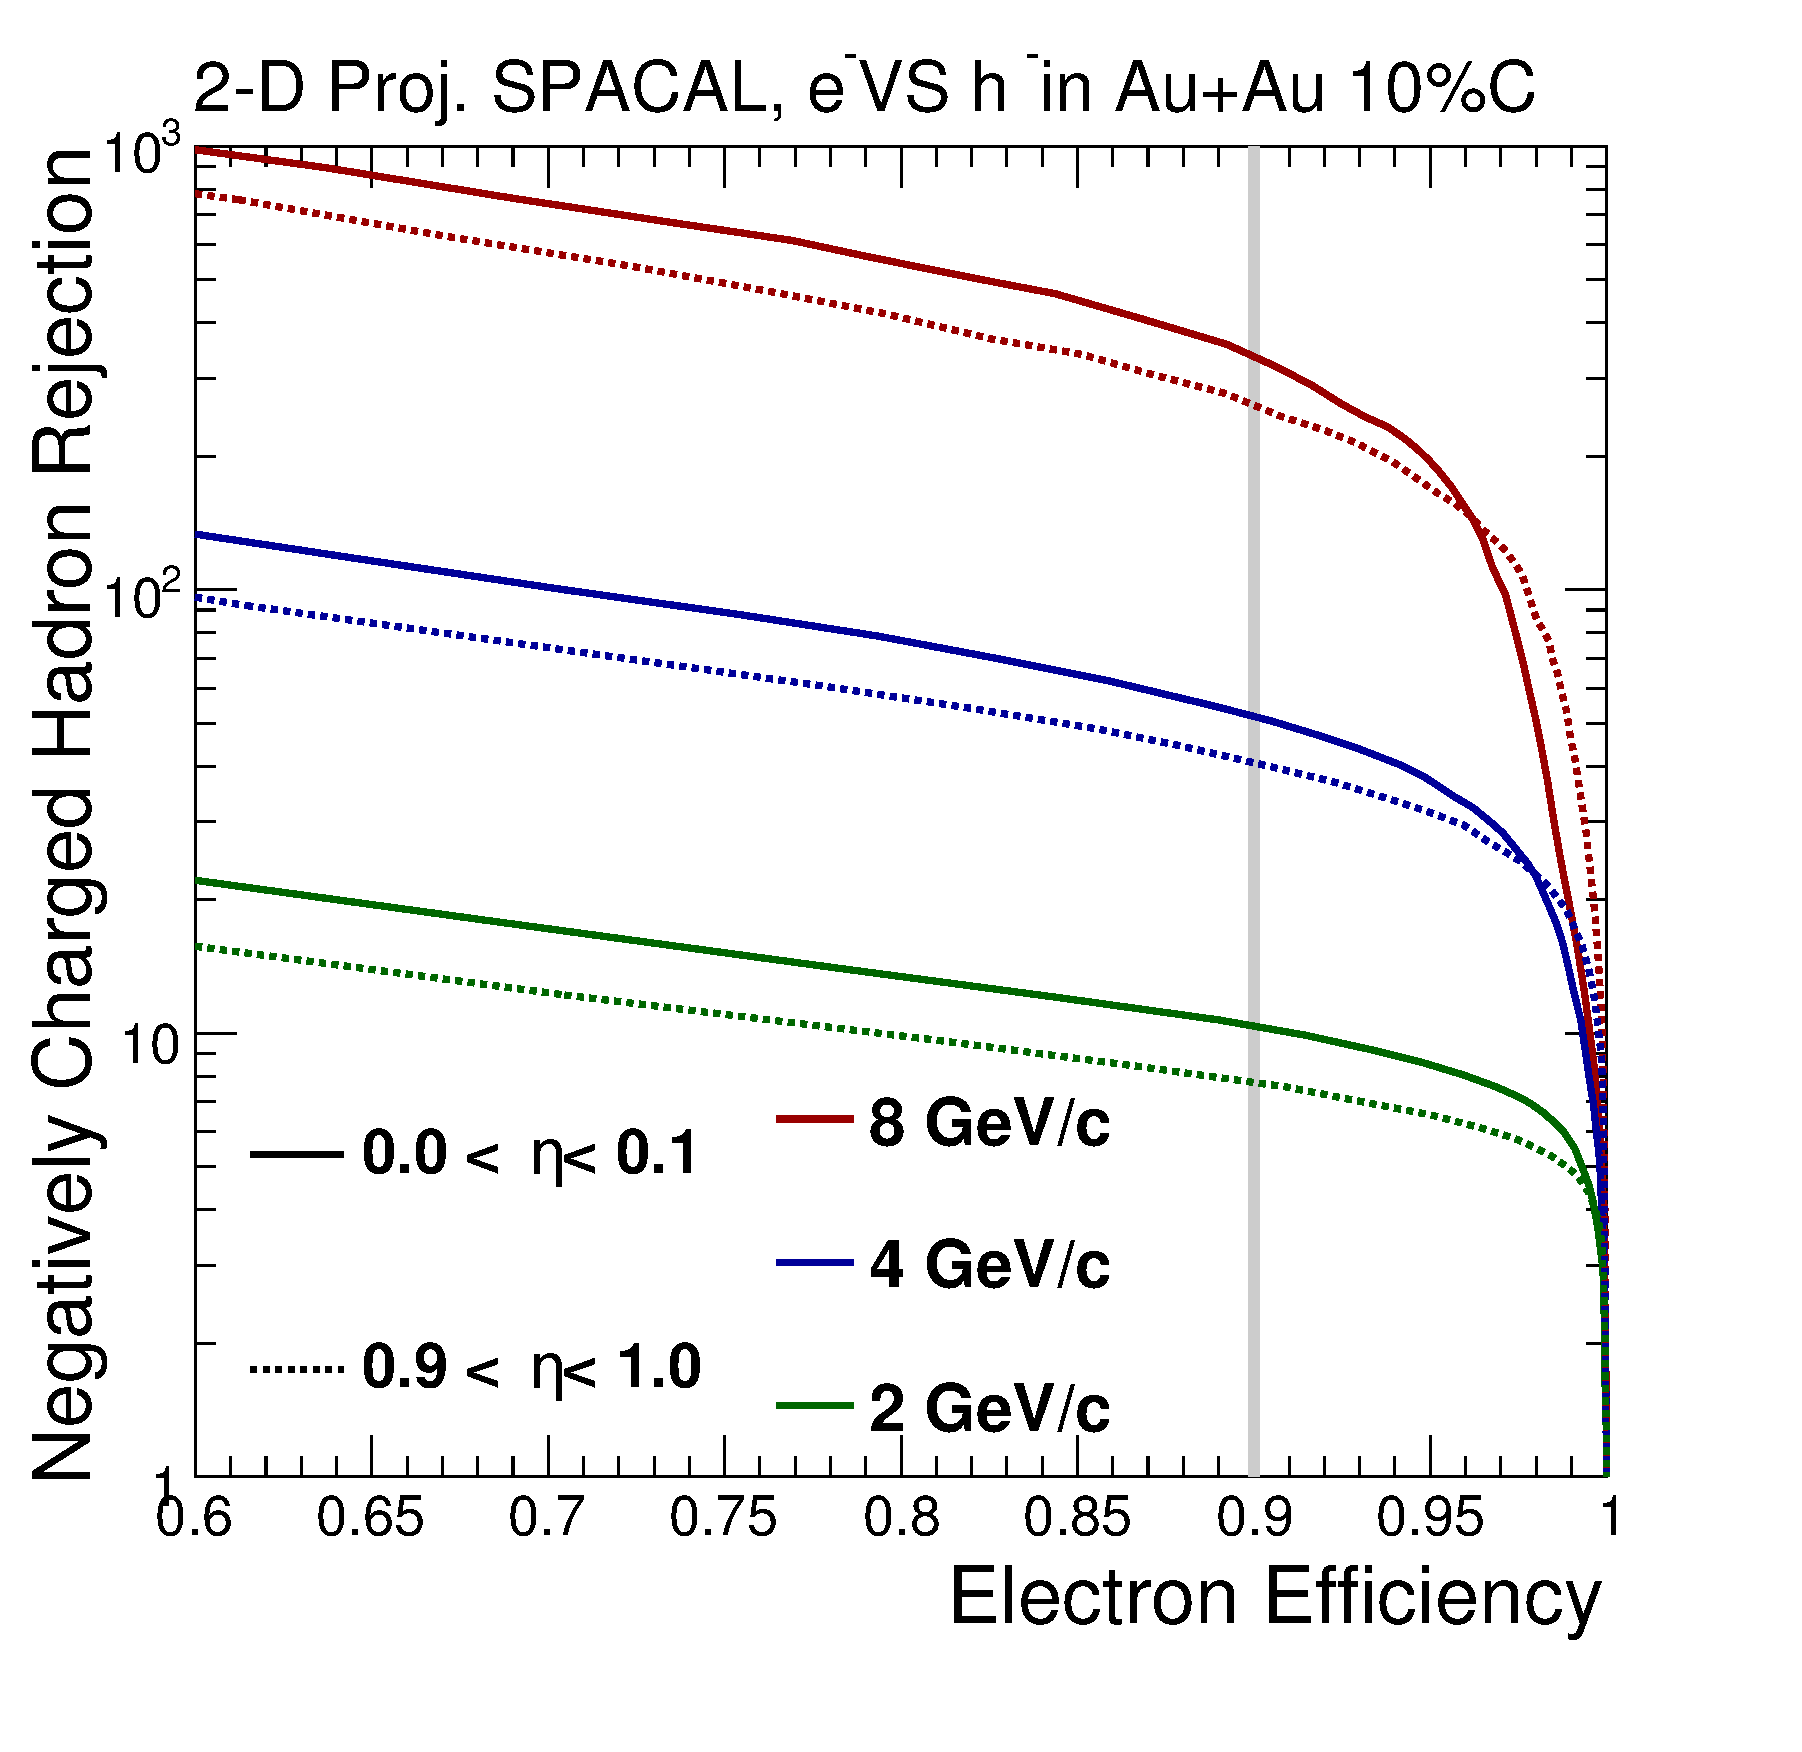
\includegraphics[width=0.4\linewidth]{figs/DrawEcal_Likelihood_Sum_RejectionCurve_AuAuSummary}
  \hspace{0.1\linewidth}
  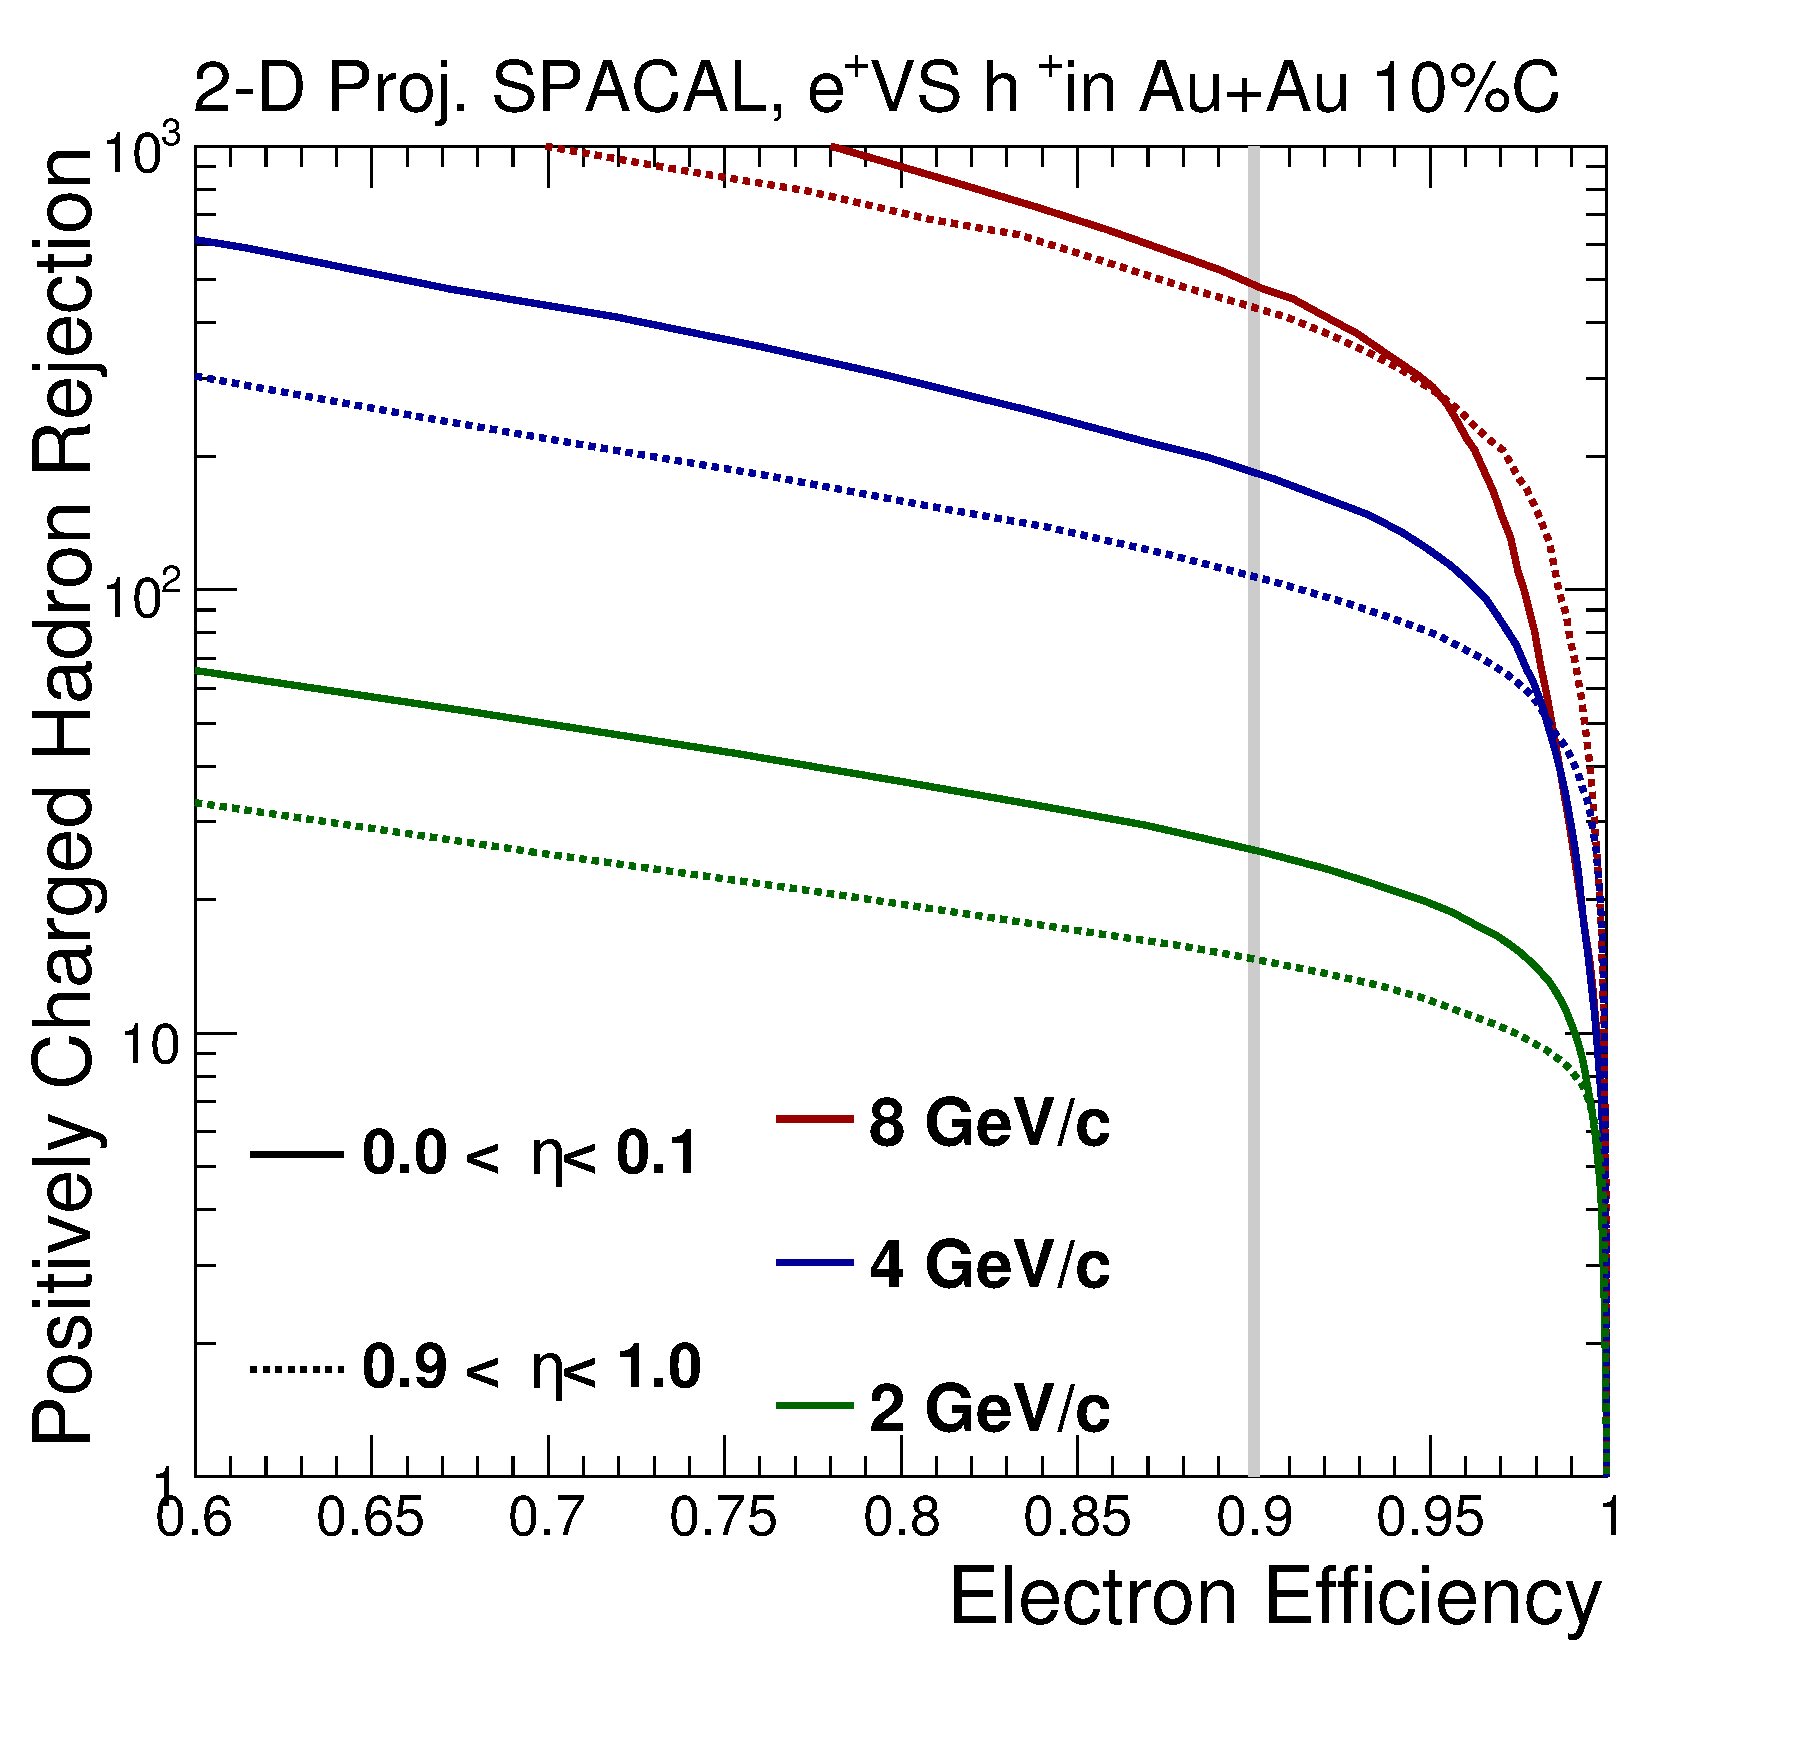
\includegraphics[width=0.4\linewidth]{figs/DrawEcal_Likelihood_Sum_RejectionCurve_AuAuSummaryPos}
  \caption{For a $2\times2$ ganged EMCal (with inner HCal present)
    inclusive charged hadron rejection is plotted on the left (right)
    as function of electron ID efficiency, for negatively (positively)
    charged tracks of three choices of momentum and for middle and
    edge rapidity in 10\% most central Au+Au events.}
  \label{fig:eid_auau}
\end{figure}

\begin{figure}[hbt]
  \centering
  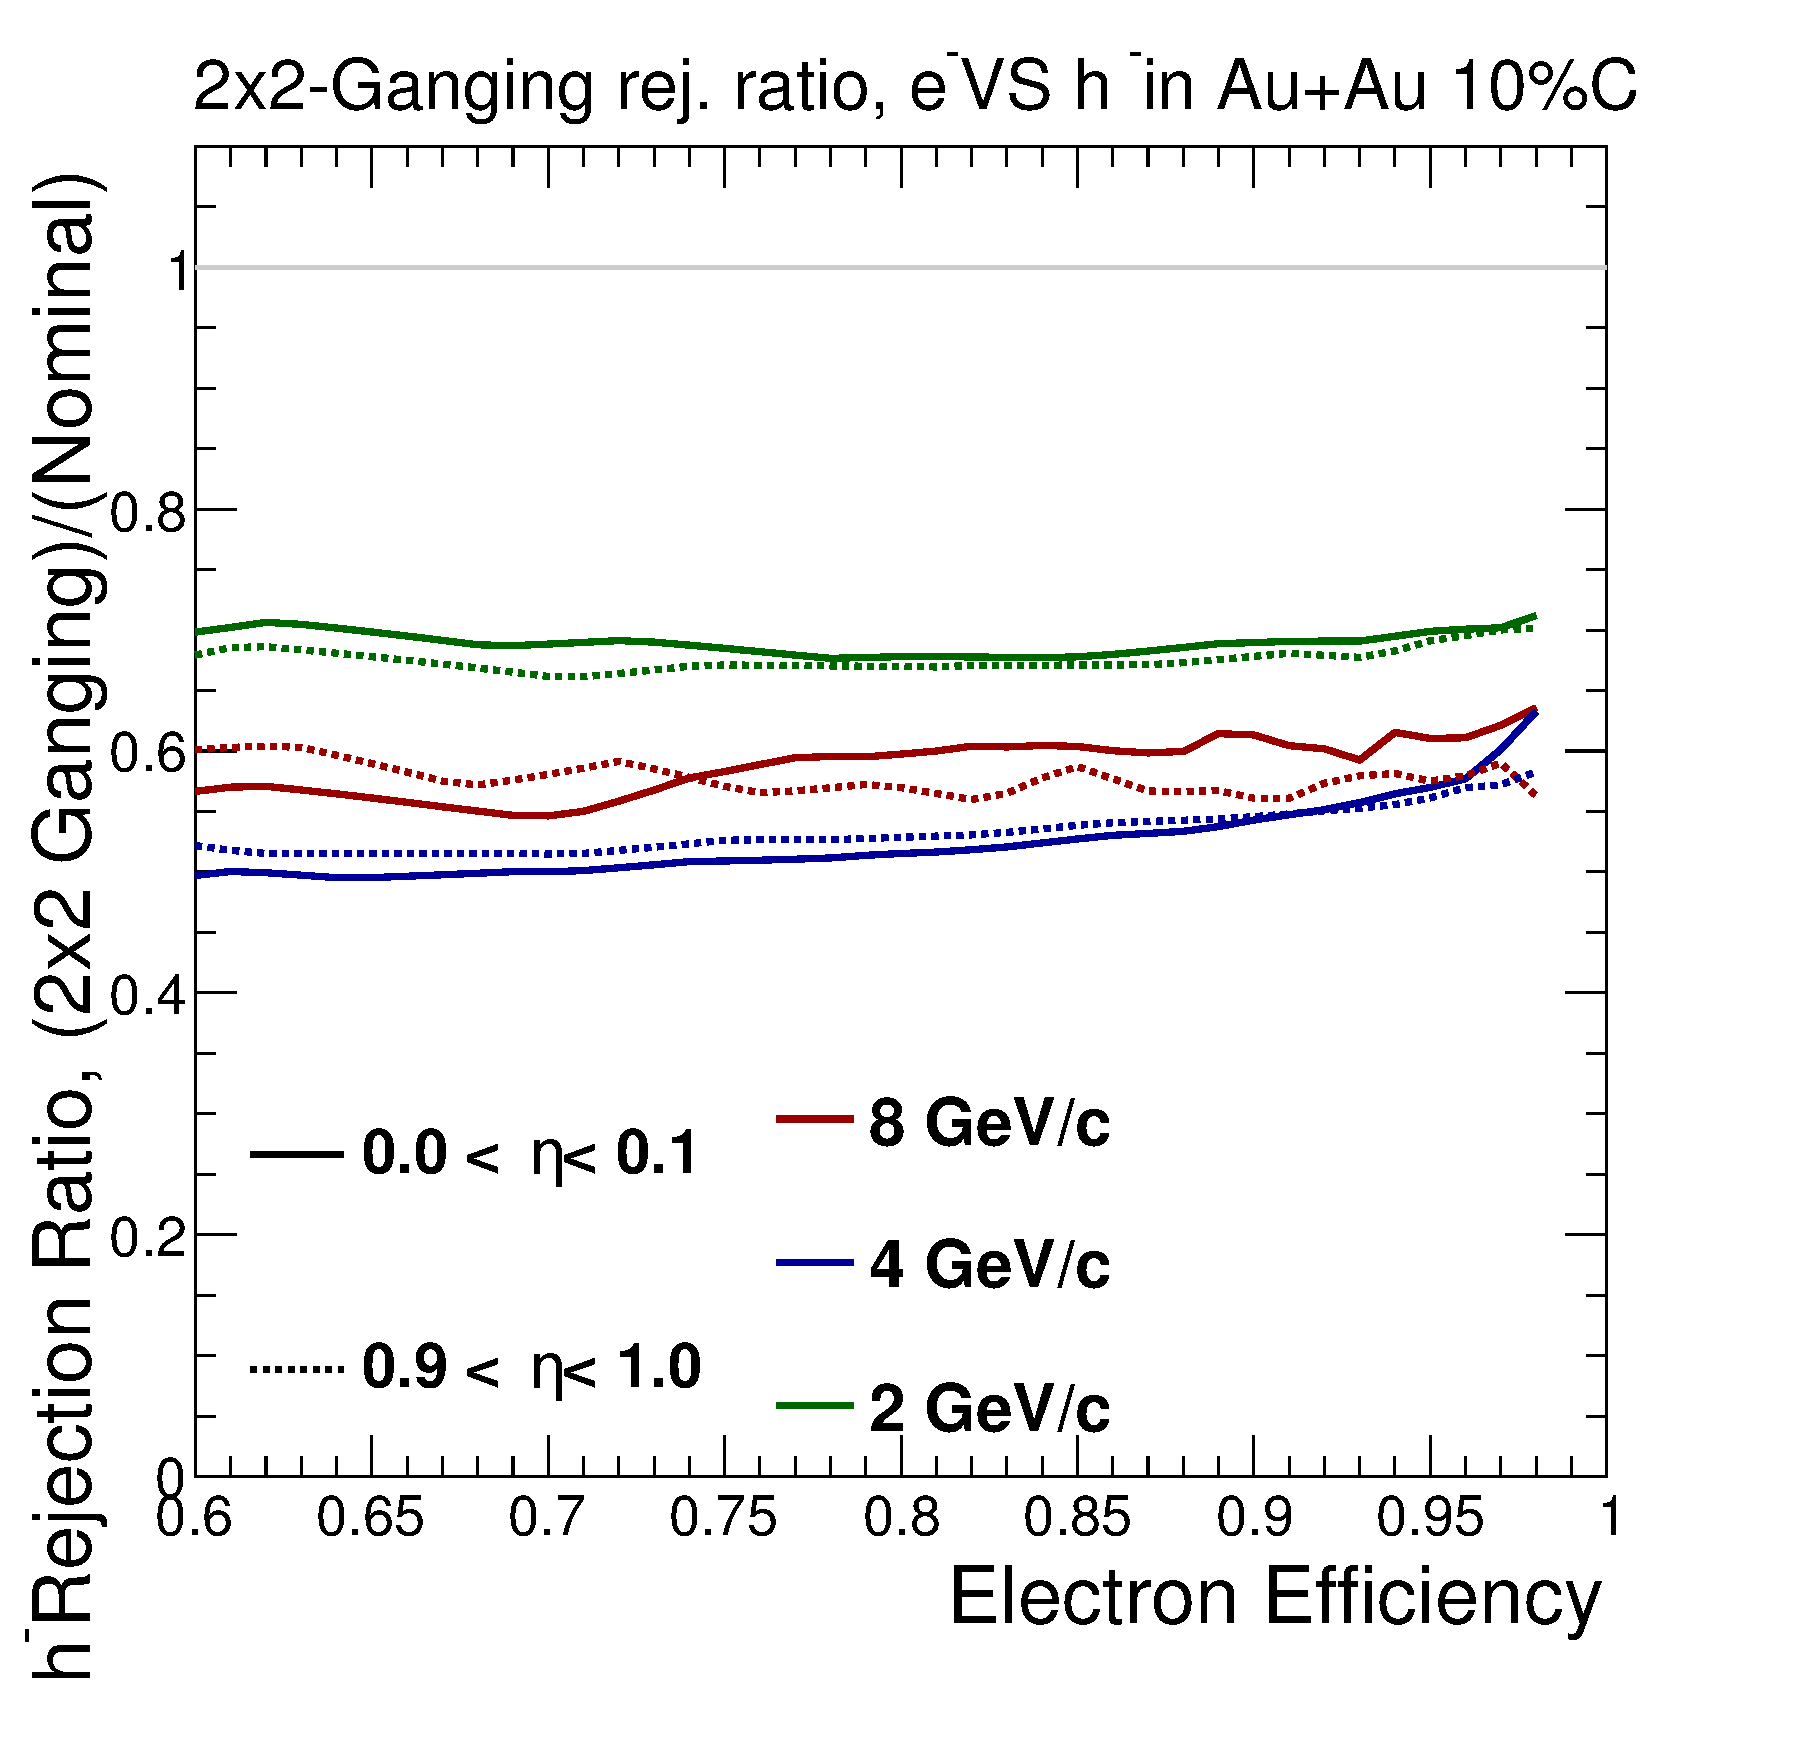
\includegraphics[width=0.5\linewidth]{figs/DrawEcal_Likelihood_Sum_RejectionCurve_AuAuSummary_Compare}
  \caption{ Ratios of inclusive charged hadron rejection of $2\times2$
    ganged EMCal to the reference design, as functions of electron ID
    efficiency. This is evaluated for negatively charged tracks of
    three choices of momentum and for middle and edge rapidity in 10\%
    most central Au+Au events.}
\label{fig:eid_ratios_auau}
\end{figure}

\begin{figure}[hbt]
  \centering
  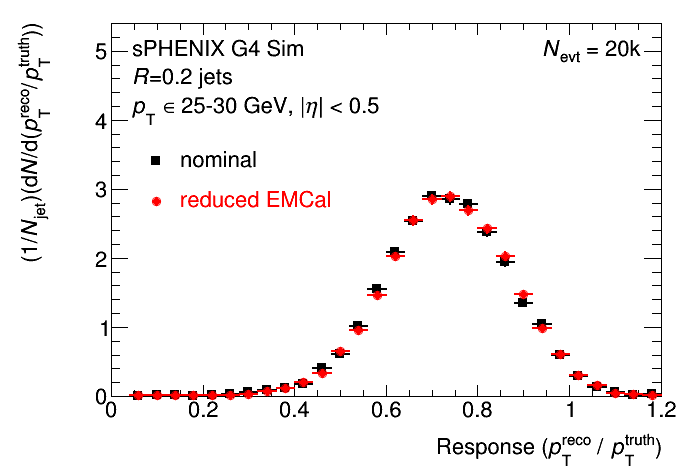
\includegraphics[width=0.5\linewidth]{figs/jet_response_reduced_emcal_eta_0} \\
  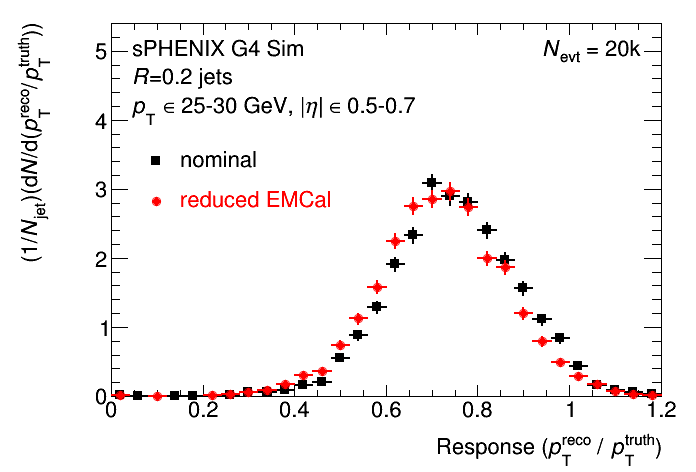
\includegraphics[width=0.5\linewidth]{figs/jet_response_reduced_emcal_eta_05} \\
  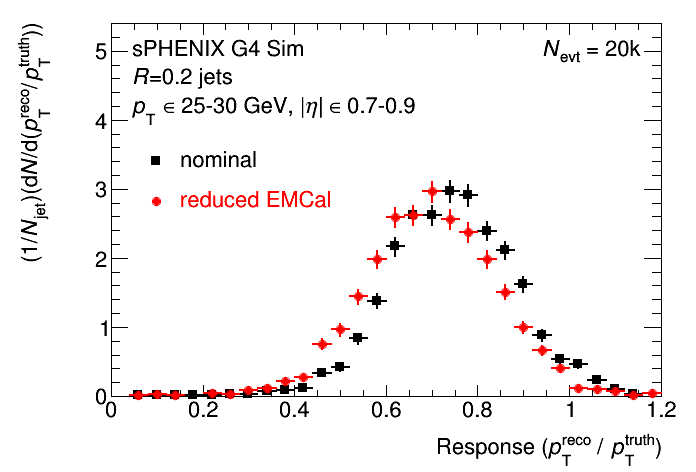
\includegraphics[width=0.5\linewidth]{figs/jet_response_reduced_emcal_eta_07}
  \caption{The effect on the jet response on reducing the EMCal to an
    acceptance within $|\eta|<0.6$ was also examined with full \geant
    simulations.  (top) The jet response for $R = 0.2$ jets near $\eta
  = 0$. (middle) The jet response for $R = 0.2$ jets near $\eta
  = 0.6$. (bottom) The jet response for $R = 0.2$ jets near $\eta
  = 0.8$.}
  \label{fig:jet_response_reduced_emcal}
\end{figure}


